\section{Introduction}

We take it the reader knows Rubin observatory (formerly LSST) and its goals. For details on the observatory and the science goals please see \cite{2008arXiv0805.2366I}. Because the name has recently changed one may still see LSST where it should say Rubin observatory, especially in reference material.

From 2018 to now  the software landscape on the Rubin Observatory construction project has changed dramatically.  We are transitioning from siloed software teams to a  more integrated approach.  The project has LabView, C++, Python and Java components - these are built in different ways and do not employ the same test harnesses. We are attempting to align all build/testing on Jenkins, although this is challenging for LabView for example. In Data Management all testing is done via pytest, all C++ code is exposed to Python so we may test it all in the python layer.  Since we have a common access layer to all Telescope control components (OpenSplice) we could follow the same approach there.
Next we are approaching deployment on the summit. To date deployments in telescope control have been fairly manual. As we shifted more toward Python, containers became more prevalent. Now most components can be deployed with Docker and Docker compose. The next logical step for them is to move to Kubernetes; this may not be possible for the camera control system but we will try to pursue this as much as possible. Data Management is already deploying the Science Platform using Kubernetes. Though the processing software for data releases is containerized it is not yet utilized in that manner.
Finally the bare metal provisioning is not fully automated - we have successfully experimented with Foreman and Puppet to bring up new blades in a selected manner. Our approach here is to provision to Kubernetes as much as possible but for other specific machines, such as camera control, to at least provision the machine with Puppet to the level needed by the camera control system.
There are strong management/cultural issues in bringing these efforts together. These are prevalent in all large projects and some of these issues will be touched on in the talk also.

\section{Background }\label{sect:back}

Rubin observatory  data management \citep{2015arXiv151207914J} has the most software by lines of code and number of people working on it in the observatory. This code is for the system to produce and allow access to the Rubin Observatory Legacy Survey of Space and Time \cite{LSE-163}.
The tools and development process of the data management team have evolved and become well honed since the official star to of the project tin 2014 \citep{2018SPIE10707E..09J}
The next large team is  Telescope and site  \citep{2014SPIE.9145E..1AG} whose software team are responsible for all the control systems on the summit. They either produce or procure each software system and integrate it with the others.
The Rubin Observatory LSST camera \citep{2010SPIE.7735E..0JK} also has a software control system and a readout system. The control system adhere to the agreed telescope and site interface.
 Bringing up the end but underpinning all of this is the IT group, which itself has two parts: one in tucson and the other in Chile.
 Across all of Rubin Observatory the systems engineering team \citep{2014SPIE.9150E..0MC} put in place guidelines and rules. They also drive the  System verification and validation: \citep{2014SPIE.9150E..0NS}.

In 2014 when the project officially started these groups were set up semi independantly, system engineering had some guidelines but these were not necessarily followed. IT was not put in a strong position in the construction site and was under staffed.This redulted in multiple problems. For example Camera and DM investigated deployment technologies comming to differnt conclusions (puppet/chef), this should have been driven by IT but IT was not envisioned as underpinning a large  modern software production.

On a positive note some sucess was had in February 2020 with AuxTel comming on sky \citep{Ingraham20}.


\section {Cyber Infrastructure Stack} \label{sect:cis}

The general Cyber Infrastructure approach of Rubin Observatory is layered as in Figure \ref{fig:ci}.
This figure came out of a broader discussion duirng the petabytes to science workshop \citep{2019arXiv190505116B}.


%\begin{figure}
%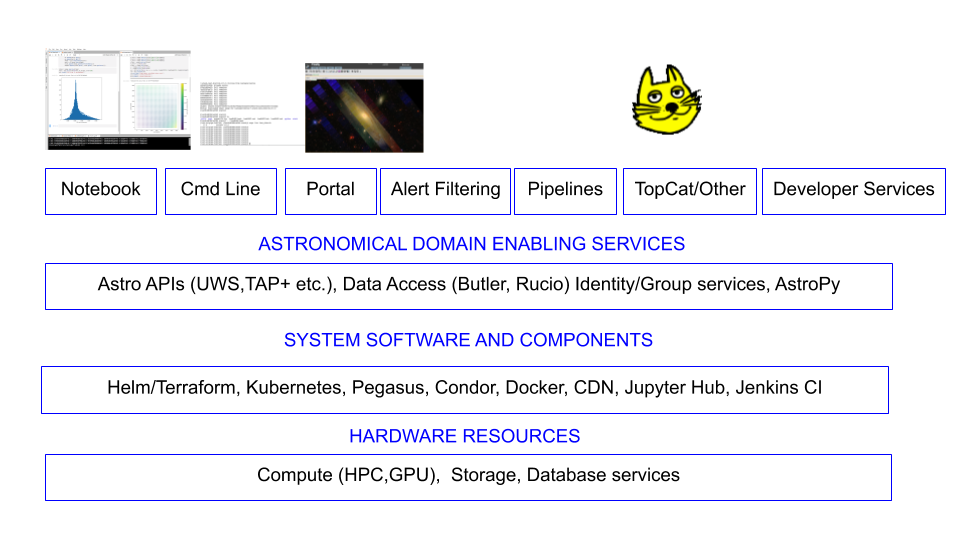
\includegraphics[width=0.6\textwidth]{CI-LSST}
%\caption{Vera C. Rubin Observatory idealized cyber infrastructure stack.} \label{fig:ci}
%\end{figure}

We aim to build a modern approach to IT just close enough to the cutting edge to allow us remain current at the start of operations but preferably not quite the bleeding edge.
The traditional approach must be augmented an element of research and development in the IT team.
This team underpins our software deployments and must be repected and trusted by developers to provide a
good underlying infrastructure.

This underlying infrastructure is considered to be a service architecture based on using standard reusable software from many of the established standards developed outside of astronomy (e.g., common authentication mechanisms such as CILogon, standard data and metadata management systems). Standard API interfaces should also be used to expose these components to higher level APIs. Data formatting and metadata structure can be exposed at the service level, allowing for more data and metadata reuse.



\section{Agnostic data access}

An example of a storage agnostic data/metadata layer is the Rubin Observatory  data butler \citep{2018arXiv181208085J}.
Creation has been driven by the need to abstract data access away from algorithms.
The algorithm code deals with Python objects and never directly with data formats or even storage.
The data butler is a lot more than a data access layer, it includes a full registry of all data objects and how to locate them.
This means it may sit atop a filesystem or an object store — an S3 plugin is now available and we are testing it in a pipeline.
The data butler is astronomy oriented — it has a built in understanding of certain relationships such as between observations and calibrations or between observations and region of the sky.
Since all metadate is held in a registry provenance queries can be answered by the butler and it already can act as the registry to find objects in an object store.

